\documentclass[14pt]{beamer}
\usepackage[T1]{fontenc}
\usepackage[utf8]{inputenc}
\usepackage[french]{babel}
\usepackage{enumerate,float,indentfirst}
\usepackage{multicol}
\usepackage{graphicx}

\usepackage[font=scriptsize]{caption} % Légende des images
\setbeamerfont{caption name}{size=\scriptsize}

\graphicspath{{images/}}

\usetheme{Pittsburgh} %Pittsburgh Boadilla
\usecolortheme{whale}
\usecolortheme{orchid}

\defbeamertemplate{description item}{align left}{\insertdescriptionitem\hfill}

\addtobeamertemplate{navigation symbols}{}{%
    \usebeamerfont{footline}%
    \usebeamercolor[fg]{footline}%
    \hspace{1em}%
    \insertframenumber/\inserttotalframenumber
}

% Permet l'affichage du Plan en début de chaque section
\AtBeginSection[]{
  \begin{frame}[shrink]{Plan}
  \small \tableofcontents[currentsection,hideothersubsections]
  \end{frame} 
}


% ************************************************
% ******************* Titre **********************
% ************************************************
\title{Images Numériques}
% \subtitle{}
\author{Jean-luc Barat}
\vspace{50pt}
\date{Novembre 2014}

% *********************** DOCUMENT ************************ %
\begin{document}
\maketitle


% ************************************************
% ******************* Sommaire *******************
% ************************************************\section*{Sommaire}
\begin{frame}[shrink]{\secname} %allowframebreaks
%  \begin{multicols}{2}
    \tableofcontents[subsectionstyle=hide]
%  \end{multicols}
\end{frame}


% **************************** Section *************************** %
\section{Introduction}
% **************************************************************** %


% ************************************************
% ******************* Diapo 1 ********************
% ************************************************
\subsection{Lumière}
\begin{frame}{\subsecname}
    La lumière est une forme d'énergie.\\
    La couleur de la lumière est caractérisée par sa fréquence.\\
    Rayonnement monochromatique / polychromatique.\\
    \textbf{Spectre} : ensemble des longueurs d'ondes d'un rayonnement polychromatique.\\
    L'oeil humain a une vision globale des composantes d'un rayonnement.\\
    ~\\
    \begin{figure}
    \centering
    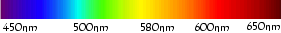
\includegraphics{spectre_visible}
    \caption{Spectre visible}
    \end{figure}
\end{frame}


% ************************************************
% ******************* Diapo  ********************
% ************************************************
\subsection{Synthèse}
\begin{frame}{\subsecname}
Deux types de synthèse de couleur :\\~\\

    \begin{table}[h]
        \centering
        \begin{tabular}{cc}
            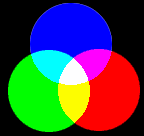
\includegraphics[width=100px]{synthese_additive}
            &
            
\includegraphics[width=100px]{synthese_soustractive}\\
            Synthèse additive & Synthèse soustractive\\
        \end{tabular}
    \end{table}
\end{frame}


% ************************************************
% ******************* Diapo  ********************
% ************************************************
\begin{frame}{\subsecname}
\begin{itemize}
    \item Additive :
        \begin{itemize}
        \item ajout de composantes à l'émission;
        \item rouge, verte, bleue;
        \item blanc : somme;
        \item noir : absences.
        \end{itemize}
    \item Soustractive :
        \begin{itemize}
        \item restitue à partir d'une source de lumière blanche;
        \item soustraction grâce à des filtres;
        \item filtres : cyan, magenta, jaune;
        \item noir : superposition;
        \item blanc : absence.
        \end{itemize}
\end{itemize}
\end{frame}


% ************************************************
% ******************* Diapo  ********************
% ************************************************
\subsection{Représentation de la couleur}
\begin{frame}{\subsecname}
    \begin{alertblock}{Problématique}
        Représentation fiable de la couleur, cohérence entre périphériques.\\
    \end{alertblock}
    \vfill
    \begin{block}{Espace de couleur}
        Représentation mathématique d'un ensemble de couleur.\\
        Différents codages : RGB, TSL, CMJN, Cie/Lab
    \end{block}
\end{frame}


% ************************************************
% ******************* Diapo  ********************
% ************************************************
\begin{frame}[allowframebreaks]{\subsecname}
\begin{block}{\textbf{gamut} ou \textbf{espace colorimétrique}} 
    Spectre de couleur d'un périphérique d'affichage.
\end{block}

\begin{figure}
    \centering
    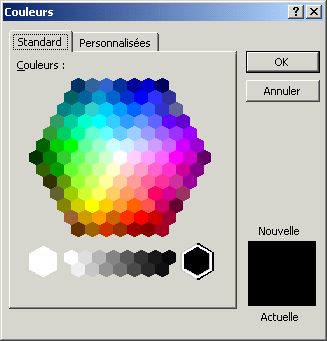
\includegraphics[height=120px]{image_nuancier}
    \caption{Nuancier d'un logiciel graphique}
\end{figure}

\end{frame}


% ************************************************
% ******************* Diapo  ********************
% ************************************************
\begin{frame}{\subsecname}
\textbf{Facteur gamma} : caractère non linéaire de l'intensité lumineuse.
\\~\\
\textbf{Gestion de la couleur} : ensemble d'opérations garantissant la conservation des couleurs d'une image dans une chaîne numérique.
\\~\\
\textbf{L'étalonnage} profil ICC (international Color Consortium). \\
%Ce profil ICC est intégré à l'image et véhicule l'ensemble des transformations subies dans la chaîne de traitement.
\end{frame}


% **************************** Section *************************** %
\section{Codages}
% **************************************************************** %


% ************************************************
% ******************* Diapo  ********************
% ************************************************
\subsection{Cie/Lab}
\begin{frame}{Codage \subsecname}
%Couleurs perçues/affichées différemment selon les individus/périphériques.\\
Standards de la CIE.%, couleurs basées sur la perception de l'oeil humain définies indépendamment des périphériques.
\begin{figure}
\centering
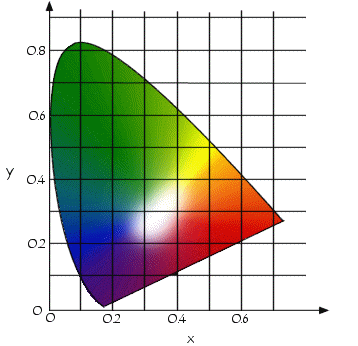
\includegraphics[height=100px]{image_cie}
\caption{Représentation graphique du modèle CIELab}
\end{figure}
\end{frame}


% ************************************************
% ******************* Diapo  ********************
% ************************************************
\begin{frame}{Codage \subsecname}
Trois modèles depuis 1931 dont le dernier Lab en 1976 :
\begin{description}
\item[L :]luminance (pourcentage, 0: noir)
\item[a :]vert au rouge (valeurs +/-120)
\item[b :]bleu au jaune (valeurs +/-120)
\end{description}

\begin{itemize}
\item Spectre visible, codages RGB et CMJN.
\item Répandu dans l'industrie.
\item Difficile à manipuler.
\item Couleurs garanties.
\end{itemize}
\end{frame}


% ************************************************
% ******************* Diapo  ********************
% ************************************************
\subsection{RVB}
\begin{frame}{Codage \subsecname}
\begin{itemize}
\item Mis au point en 1931 par la CIE.
\item Trois rayonnements monochromatiques.
\item Représentation informatique.
\item Composante codée sur un octet.
\end{itemize}
\begin{figure}
\centering
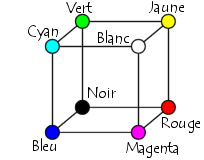
\includegraphics[height=80px]{image_rgb}
\caption{Représentation graphique du codage}
\end{figure}
\end{frame}


% ************************************************
% ******************* Diapo  ********************
% ************************************************
\subsection{TSL}
\begin{frame}[allowframebreaks]{Codage \subsecname}
    \vfill
    \begin{itemize}
    \item Albert H.Munsell.
    \item Représentation naturelle.
    \item Mis au point afin permettre un choix interactif.
    \item Non adapté à la description quantitative d'une composante.
    \end{itemize}
    \vfill
    \begin{figure}
    \centering
    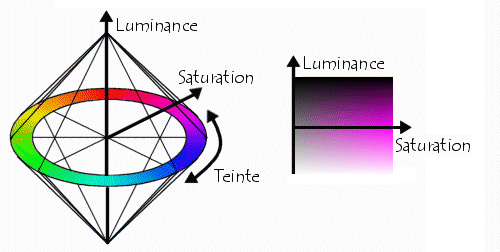
\includegraphics[height=100px]{image_tsl}
    \caption{Représentation graphique du modèle TSL}
    \end{figure}
    \begin{description}
    \item[Teinte]: perception de la couleur.
    \item[Saturation]: pureté la couleur (vif ou terme)
    \item[Luminance]: quantité de lumière de la couleur
    \end{description}
\end{frame}


% ************************************************
% ******************* Diapo  ********************
% ************************************************
\subsection{CMJN}
\begin{frame}{Codage \subsecname}
    \begin{itemize}
    \item Décomposition de la lumière.
    \item Synthèse soustractive.
    \item Blanc : absence.
    \item Noir (partiel) : superposition.
    \end{itemize}
    \begin{figure}
    \centering
    
\includegraphics[width=50px]{synthese_soustractive}
    \caption{Synthèse soustractive}
    \end{figure}     
    + noir (pur) $\rightarrow$ quadrichromie / CMJN.
\end{frame}


% **************************** Section *************************** %
\section{Images}
% **************************************************************** %


% ************************************************
% ******************* Diapo  ********************
% ************************************************
\subsection{Codage des images}
\begin{frame}{\subsecname}
%\item[Infographie] : domaine informatique concernant la création et la manipulation d'images numériques.
\begin{block}{Image numérique}
Ensemble de points (tableau 2D).
\end{block}
\begin{block}{Pixel (PICture ELement)}
Plus petit élément constitutif d'une image numérique.
\end{block}

\begin{figure}
\centering
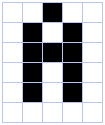
\includegraphics[height=75px]{image_pixels}
\caption{Représentation de pixels}
\end{figure}
\end{frame}


% ************************************************
% ******************* Diapo  ********************
% ************************************************
\begin{frame}{Définition et Résolution}

\begin{block}{Définition}
Nombre de pixels constituant l'image.
\end{block}
\vfill
\begin{block}{Résolution}
Nombre de pixels par unité de surface (PPP/DPI).
\end{block}
\end{frame}


% ************************************************
% ******************* Diapo  ********************
% ************************************************
\begin{frame}{Codage de la couleur}
    Image représentée par un tableau à deux dimensions dont chaque case est un pixel.
    \begin{block}{Profondeur des couleurs}
    Nombre de bits représentant la couleur/intensité d'un pixel.
    \end{block}
    \begin{block}{Palette de couleurs (colormap)}
    Ensemble de couleurs contenues dans l'image, nombre de couleurs possibles $\rightarrow$ taille du codage de l'indice.
    \end{block}
    
\end{frame}


% ************************************************
% ******************* Diapo  ********************
% ************************************************
\begin{frame}
    Quelques standards de codage :
    \begin{itemize}
    \item bitmap noir et blancs : 1 bit/px;
    \item bitmap 16 couleurs/gris : 4 bits/px;
    \item bitmap 256 couleurs/gris : 8 bits/px;
    \item image indexée : couleurs codées par palette.
    \item couleurs vraies (true color) : trois composantes par pixel  $\rightarrow$ 24bits, + transparence $\rightarrow$ 32bits.
    \end{itemize}
\end{frame}


% ************************************************
% ******************* Diapo  ********************
% ************************************************
\begin{frame}{Poids d'une image}
    \begin{block}{Poids d'une image}
    Nombre de pixels $\times$ taille de son codage.
    \end{block}
    Exemple :
    \begin{tabular}{|l|l|l|l|}
      \hline
      Définition  & Noir et blanc & 256  & True color \\ 
      & & couleurs & (24bits) \\
      \hline
      1024x768 & 96Ko & 768Ko & 2.3Mo \\
      \hline
    \end{tabular}
\end{frame}


% ************************************************
% ******************* Diapo  ********************
% ************************************************
\begin{frame}{Transparence}
    \begin{block}{Transparence}
    Niveau d'opacité des éléments d'une image.\\
    \end{block}
    \vfill
    Deux modes de transparence : 
    \begin{itemize}
    \item simple : (indexée) une couleur transparente;
    \item couche alpha : ajout d'un octet / pixel. (Alpha Blending Process).
    \end{itemize}
\end{frame}


% ************************************************
% ******************* Diapo  ********************
% ************************************************
\subsection{Bitmap vs vectoriel}
\begin{frame}{\subsecname}
    \begin{block}{Image bitmap (raster)}
        Image pixelisée.
    \end{block}
    \vfill

    \begin{description}
    \item[Distorsion] : perte d'information.
    \item[Pixellisation] : apparition de "pixels".
    \end{description}
\end{frame}


% ************************************************
% ******************* Diapo  ********************
% ************************************************
\begin{frame}
    \begin{block}{Image Vectorielle}
        Représentation par formules mathématiques d'entités géométriques.\\
    \end{block}
    \vfill
    \begin{itemize}
    \item Calcul des entités à chaque modification.
    \item Modifiable sans perte d'information.
    \item Fichier peu volumineux.
    \item Formes simples.
    \item Toutes images ne peut être transformées en image vectorielle (photographie).
    \item Technologie Macromédia Flash $\rightarrow$ sites internet.
    \end{itemize}
\end{frame}


% ************************************************
% ******************* Diapo  ********************
% ************************************************
\begin{frame}
    \begin{table}[h]
        \begin{tabular}{|c|c|}
            \hline
            
\includegraphics[width=130px]{image_rond_mat}
            &  
            
\includegraphics[width=130px]{image_rond_vect}\\
            \hline
            Représentation & Représentation\\
            image matricielle & image vectorielle\\
            \hline
        \end{tabular}
    \end{table}
\end{frame}


% ************************************************
% ******************* Diapo  ********************
% ************************************************
\subsection{Formats graphiques}
\begin{frame}{\subsecname}
    Codage affichage $\neq$ codage stockage.\\
    Compression $\rightarrow$ gain de mémoire.\\
    Modifications sans pixelisation $\rightarrow$ stockage d'équations.\\
    Fichier > processeur > carte graphique > moniteur.
    \begin{tabular}{|l|l|l|l|}
    \hline
    Format & Compression & Dim. max. & Couleurs \\
    \hline
    SVG & textuel & 2\up{16}x2\up{16} & 2\up{24} \\
    \hline
    BMP & aucune / RLE & 2\up{16}x2\up{16} & 2\up{24} \\
    \hline
    GIF & LZW & 2\up{16}x2\up{16} & 2\up{8} \\
    \hline
    PNG & RLE & 2\up{16}x2\up{16} & >2\up{24} \\
    \hline
    TIF & \small{RLE/LZW/JPEG ...} & 2\up{32}-1 & >2\up{14} \\
    \hline
    \end{tabular}
\end{frame}



% ************************************************
% ******************* Diapo  ********************
% ************************************************
\subsection{SVG}
\begin{frame}[allowframebreaks]{Le format \subsecname~scalable Vector Graphics}
    \begin{figure}
    \centering
    
\includegraphics[height=100px]{image_bitmap_svg}
    \caption{Image bitmap vs. vectorielle}
    \end{figure}
    \begin{itemize}
        \item Format d'image graphique vectoriel.
        \item Conçu en 1999 basé sur XML et inspiré du VML (Microsoft) et PGML (Adobe).
        \item Spécifié par le W3C.
        \item Décrit des ensembles de graphiques vectoriels.
        %\item Coordonnées, dimensions et structures des objets vectoriels sous forme numérique.
        \item Système de style pour couleurs et polices de caractères (CSS ou XSL).
        \item Formes géométriques de base.
        \item Chemins, courbes de Bézier.
        \item Dégradés et couleurs de motif (SVG quelconques).
        \item Transparence.
    \end{itemize}
\end{frame}



% ************************************************
% ******************* Diapo  ********************
% ************************************************
\subsection{BMP}
\begin{frame}{Le format \subsecname}
Format d'image graphique simple (Microsoft/IBM).
\begin{itemize}
\item Pixels stockés sous forme de tableau de points.
\item Couleurs vraies, palette indexée.
\item Indépendant du périphérique d'affichage.
\item Codage : suite de bits (bas gauche).
\end{itemize}
\vfill
Exemples :
\begin{itemize}
\item image en 2 couleurs : 1bit/px $\rightarrow$ 8px/octet;
\item image en 16 couleurs : 4bit/px $\rightarrow$ 2px/octet;
\item couleurs réelles : 24bits/px.
\end{itemize}

% Structure d'un fichier
% L'en-tête du fichier
% informations sur le type de fichier (Bitmap).
% Taille du fichier (en octets), 
% L'offset de l'image : adresse relative des informations de l'image par rapport au début du fichier.

% L'entête de l'image (entre autres)
% Taille totale (octets).
% Largeur et longueur (pixels).
% Résolution horizontale et verticale (pixels/m).
% Compression.
% Nombre de couleur de la palette.

% La palette (optionelle) 
% 4 octets par entrée : composantes (1 octet) bleue, verte, rouge.

%Chaque ligne de l'image doit comporter un nombre total d'octets multiple de 4 (complétée par des 0).
\end{frame}


% ************************************************
% ******************* Diapo  ********************
% ************************************************
\subsection{GIF}
\begin{frame}{GIF : Graphic Interchange Format}
    Format graphique bitmap (Compuserve).
    \begin{itemize}
    \item 2 à 256 couleurs dans sa palette. 
    \item Fichier de taille très faible.
    \item Compression LZW (Unisys).
    \end{itemize}
    \begin{itemize}
    \item GIF 87 :
        \begin{itemize}
        \item entrelacement;
        \item animation.
        \end{itemize}
    \item GIF 89 :
        \begin{itemize}
        \item une couleur transparente;
        \item délai pour les animations.
        \end{itemize}
    \end{itemize}
\end{frame}


% ************************************************
% ******************* Diapo  ********************
% ************************************************
\subsection{PNG}
\begin{frame}{\subsecname : Portable Network Graphic}
    \begin{itemize}
    \item Mis au point en 1995.
    \item Alternative libre au format GIF.
    \item Codage :
    \begin{itemize}
        \item noir et blanc (<16 bits/pixel);
        \item couleurs réelles (<48 bits/pixel);
        \item indexées (palette 256 couleurs).
    \end{itemize}
    \item Transparence.
    \item Entrelacement.
    \item Compression sans perte.
    \end{itemize}

% Structure du fichier 
% signature  identifiant le fichier comme un fichier PNG.
% série d'éléments nommés \textit{chunks} (segments).
% chaque segment est composé de quatre parties
% sa taille (  entier non signée de 4 o)
% son type ( 4 o code de quatre caractères  ASCII)
% les données du segment
% le CRC ( code correcteur de 4 o)

%     les principaux segments (critical chunks) 
%     \begin{itemize}
%     \item Image header (IHDR)
%     \item Palette (PLTE)
%     \item Image data (IDAT)
%     \item Image Trailer (IEND)
%     \end{itemize}
    
% D'autres segments (anciliary chunks) permettant de coder par exemple la couleur de fond, les gammas, la transparence. 
\end{frame}



% ************************************************
% ******************* Diapo  ********************
% ************************************************
\subsection{TIF}
\begin{frame}[allowframebreaks]{\subsecname : Tagged Image File Format}
    Balises caractérisant l'image (dimensions, nombre de couleurs, compression, ...).
    \begin{itemize}
%    \item Format de fichier graphique bitmap.
    \item Mis au point en 1987 (Aldus).
    \item Codage :
        \begin{itemize}
        \item noir et blanc;
        \item couleur réelle (32 bits/pixel);
        \item indexée de taille importante (4Go).
        \end{itemize}
    \item Sans perte de qualité.
    \item Indépendamment des périphériques/plate-formes.
    \item Espaces de couleur possibles (RGB, CMJN, ...).
    \item Programmation facile de logiciel permettant de manipuler le format. 
    \item Multiples options non reconnues dans différents lecteurs ($\rightarrow$ image illisible).
    \end{itemize}
\end{frame}



% ************************************************
% ******************* Diapo  ********************
% ************************************************
\section{Compression}
\begin{frame}{\secname}
    \begin{itemize}
    \item Réduction de la taille des données.
    \item Augmentation rapidité de transmission).
    \item Algorithme pour la compression et la décompression.
    \item Dépendant du type de fichier.
    \item Taux de compression.
    \end{itemize}
\end{frame}


% ************************************************
% ******************* Diapo  ********************
% ************************************************
\begin{frame}{Types de compressions}
    \begin{itemize}
    \item Physique et logique (données redondantes/substitution);
    \item symétrique et asymétrique : compression/décompression identique.
    \item avec pertes : meilleur taux de compression. irréversible;
    \item adaptif, semi-adaptif, non adaptif : algorithmes basés sur dictionnaires.
    \end{itemize}

\end{frame}


% ************************************************
% ******************* Diapo  ********************
% ************************************************
\subsection{RLE}
\begin{frame}{\subsecname : Run Length Encoding}
%Concaténation de point : optimisation du stockage des points.\\
%Image monochrome -> deux couleurs -> un bit / px.\\
Basé sur la répétition d'éléments consécutifs. \\
Codage par plage\\
principe : coder le nombre de répétition puis la valeur.\\
\vfill
Exemple : AAAAABBBB -> 5A4B.\\
\vfill
Plus complexe -> potentiel gaspillage.
\end{frame}



% ************************************************
% ******************* Diapo  ********************
% ************************************************
\subsection{Huffman}
\begin{frame}{\subsecname}
\begin{itemize}
\item Attribut un code binaire aux différents symboles.\\
\item Codage préfixé à longueur variable.\\
%le codeur de Huffman crée un arbre ordonné à partir des symboles et de leur fréquence d'apparition.
%Le code de chaque symbole correspond à la suite des codes le long du chemin du symbole à la racine.
\item Création d'un arbre ordonné.
\item Bon taux de compression.
\end{itemize}
\vfill
\end{frame}

\begin{frame}{\subsecname}
\begin{figure}
\centering
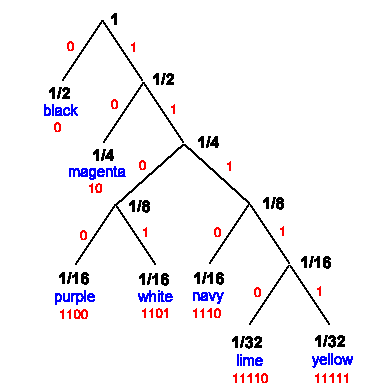
\includegraphics[height=0.7\textheight]{image_huffman}
\caption{Arbre de Huffman}
\end{figure}
\end{frame}



% ************************************************
% ******************* Diapo  ********************
% ************************************************
\subsection{LZW}
\begin{frame}{\subsecname}
\begin{itemize}
\item Inventé en 1977 (A. Lempel et J. Ziv).
\item Spécialisation compression d'image en 1978.
\item Très rapide.
\item Travail sur les bits. Dictionnaire.
\item Basé sur la multiplicité des occurrences.
%\item Principe : substitution des motifs par un indice issu de la construction d'un dictionnaire.
\item LZW Breveté.
\item PNG utilise LZ77.
\end{itemize}

\end{frame}



% ************************************************
% ******************* Diapo  ********************
% ************************************************
\subsection{JPEG}
\begin{frame}{\subsecname : Joint Photographic Expert Group}
\begin{itemize}
\item Réunion comité d'expert créé en 1986.
\item Compression avec perte. 
\item Meilleur taux de compression.
\item Très efficace sur des images photographiques.
\item Utilise RLE et Huffman.
\item Sans perte pour l'imagerie médicale.
\end{itemize}
\end{frame}



% ************************************************
% ******************* Diapo  ********************
% ************************************************
\section{Traitements graphiques}
\subsection{Traitements graphiques}
\begin{frame}{\subsecname}
\begin{block}{histogramme}
Représentation de la distribution des intensités des pixels.
\end{block}

\begin{figure}
\centering
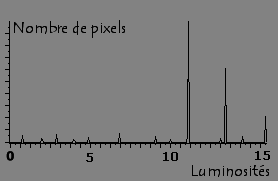
\includegraphics[width=140px]{image_histogramme}\\

\includegraphics[width=140px]{image_palette}
\caption{Histogramme}
\end{figure}
\end{frame}


\begin{frame}{\subsecname}
\begin{block}{Modification d'histogramme}
But : correction du contraste et l'échelle des couleurs pour les images sur/sous-exposées.\\
Modification non altérante des informations de l'image.
\end{block}

\begin{block}{Étirement d'histogramme}
Consiste à répartir les fréquences d'apparition des pixels sur la largeur de l'histogramme -> pixels sombres plus sombres et clairs plus claires
\end{block}
\end{frame}


\begin{frame}{\subsecname : égalisation d'histogramme}
% harmonisation de la répartition des niveaux de luminosité. augmente les nuances dans l'image.
\begin{table}[h]
\centering
\begin{tabular}{|c|c|}
\hline
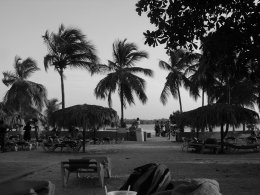
\includegraphics[width=130px]{image_exemple_plage}
&  
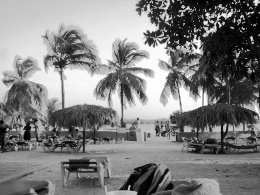
\includegraphics[width=130px]{image_exemple_plage_eq}
 \\
 \hline
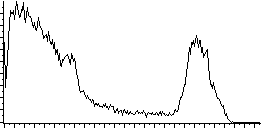
\includegraphics[width=130px]{image_exemple_plage_hist}
& 
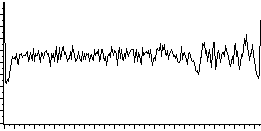
\includegraphics[width=130px]{image_exemple_plage_eq_hist}
 \\
 \hline
\end{tabular}
\end{table}
\end{frame}

\begin{frame}{\subsecname}
\begin{block}{Seuillage}
Met à zéro tous les pixels ayant une valeur inférieure à un seuil et à la valeur maximal ceux ayant une valeur supérieure.\\
\end{block}
\begin{figure}
\centering
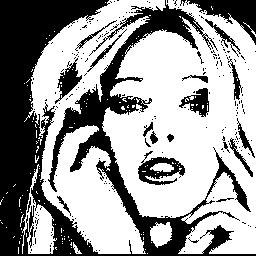
\includegraphics[width=100px]{image_femme_seuil}
\caption{Image après traitement seuil}
\end{figure}
\end{frame}



% ************************************************
% ******************* Diapo  ********************
% ************************************************
\subsection{Filtres}

\begin{frame}[allowframebreaks]{\subsecname}

\begin{block}{Filtre}
Transformation mathématique, produit de convolution. Représenté par une matrice.\\
Modifie la valeur de chaque pixel en fonction de la valeur des ceux avoisinants affectées de coefficients.\\
Image traitée : produit de la matrice image par le filtre.
\end{block}

Exemple d'un filtre 3x3 :
\begin{table}[h]
\centering
\begin{tabular}{|c|c|c|}
 \hline
 1 & 1 & 1 \\
 \hline
 1 & 4 & 1 \\
 \hline
 1 & 1 & 1 \\
 \hline
\end{tabular}
\end{table}

\begin{block}{Passe-bas}
Atténuation des fréquences hautes (pixels foncés).
\end{block}
\begin{block}{Passe-haut}
Composantes basse fréquence, accentuation des détails et contrastes.
\end{block}
\begin{block}{Filtre directionel} 
Transformation selon une direction.
\end{block}

\end{frame}


% ************************************************
% ******************* Diapo  ********************
% ************************************************
\subsection{Effets}
\begin{frame}[allowframebreaks]{\subsecname}
\begin{block}{Bruit}
Caractérise les parasites d'un signal, pixels à l'intensité très différente de celle des pixels avoisinants.\\
Provenance : acquisition.
\end{block}

\begin{block}{Lissage}
Opération visant à éliminer le bruit d'une image.\\
Anticrénelage : atténuation de l'effet escalier en bordure d'une forme.
\end{block}

\begin{block}{Accentuation}
Inverse du lissage, accentuation des différences entre pixels voisins.
Extraction de contours : limite entre zones homogènes de l'image.
\end{block}

\begin{block}{Tramage}
Technique alternant des motifs géométriques utilisant peu de couleurs pour simuler une couleur plus élaborée.
\end{block}

\end{frame}



% ************************************************
% ******************* Diapo  ********************
% ************************************************
\section{Quelques Outils}

\begin{frame}{\secname}
Logiciels pour format vectoriel
 \begin{itemize}
  \item Adobe Flash / Fireworks / Illustrator
  \item Gill (logiciel libre)
  \item OpenOffice.org Draw (logiciel libre)
 \end{itemize}
Logiciels pour format matriciel
 \begin{itemize}
  \item Adobe Photoshop
  \item Microsoft Paint
  \item GIMP
 \end{itemize}
\end{frame}

\end{document}
